\newpage % Rozdziały zaczynamy od nowej strony.

\section{Wyniki}
Wszystkie wykorzystane architektury zostały wytrenowane na zbiorze danych liczącym 50 tysięcy zdjęć wraz z jednym podpisem do każdego zdjęcia. Dane były przetwarzane w seriach liczących po 10 elementów. Przetwarzanie było powtarzane dziesięciokrotnie na całym zbiorze treningowym, natomiast wartości metryk zostały obliczone na podstawie tekstów wygenerowanych przy pomocy zbioru testowego liczącego 10 tysięcy zdjęć.

Lepsza skuteczność wiążę się z o wiele większymi wymaganiami sprzętowymi danego rozwiązania, co można zauważyć na rysunku \ref{fig:memory}, na którym zawarte są informacje o rozmiarze pamięci RAM jednostki GPU wymaganej do uruchomienia konkretnej architektury. Sieci VGG16, VIT oraz GIT przekraczają wartość 4 GB, co uniemożliwia ich uruchomienie przy pomocy karty graficznej GeForce GTX 1650, wykorzystanej w ramach eksperymentów, ponieważ posiada ona jedynie 4 GB pamięci.
\begin{figure}[H]
  \centering
  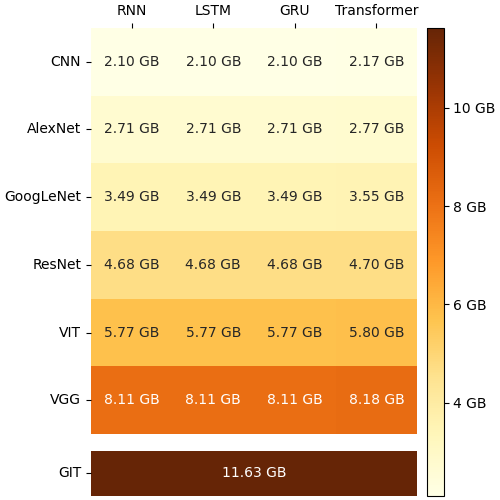
\includegraphics[width=.9\linewidth]{timings/ram}
  \caption{Pamięć RAM potrzebna do uruchomienia testowanych architektur wyrażona w gigabajtach. Opracowanie własne.}
  \label{fig:memory}
\end{figure}

\begin{figure}[H]
  \centering
  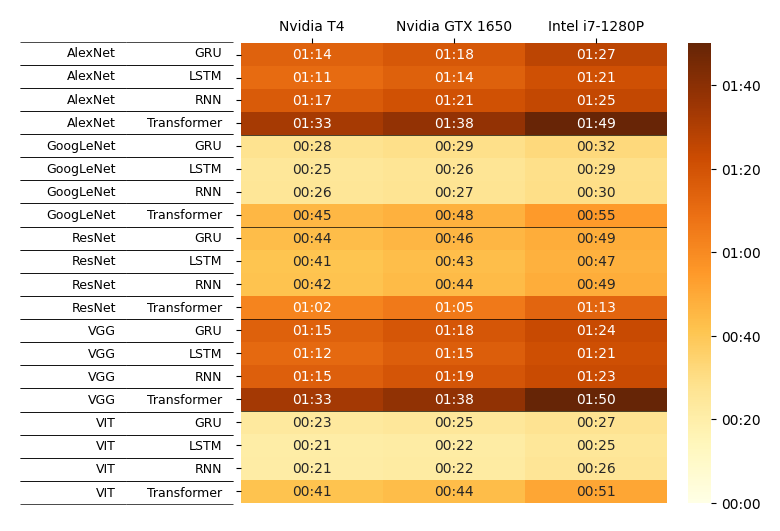
\includegraphics[width=.9\linewidth]{timings/timings_decoders}
  \caption{Czas potrzebny na przetworzenie jednej epoki treningowej poszczególnych kombinacji modułów kodujących oraz dekodujących wykorzystujących wcześniej wytrenowane moduły kodujące. Dane przedstawione w skali logarytmicznej. Opracowanie własne.}
  \label{fig:timings-decoders}
\end{figure}

\begin{figure}[H]
  \centering
  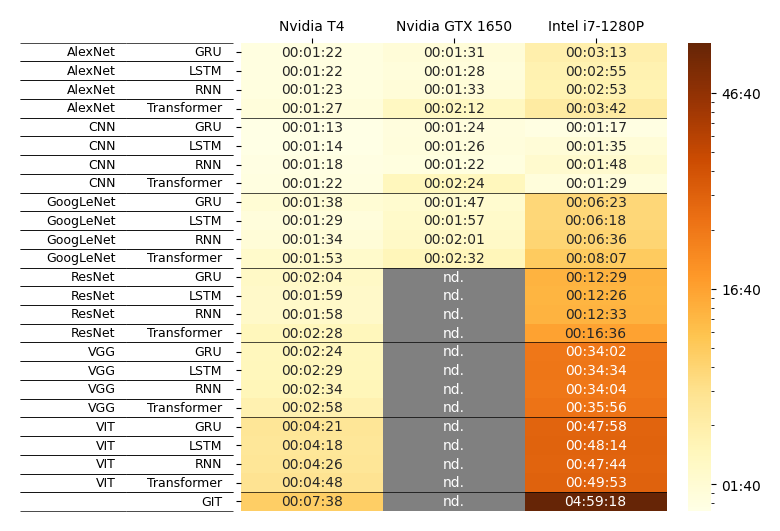
\includegraphics[width=.9\linewidth]{timings/timings_networks}
  \caption{Czas potrzebny na przetworzenie jednej epoki treningowej poszczególnych kombinacji modułów kodujących oraz dekodujących. Opracowanie własne.}
  \label{fig:timings-networks}
\end{figure}

\begin{figure}[H]
  \centering
  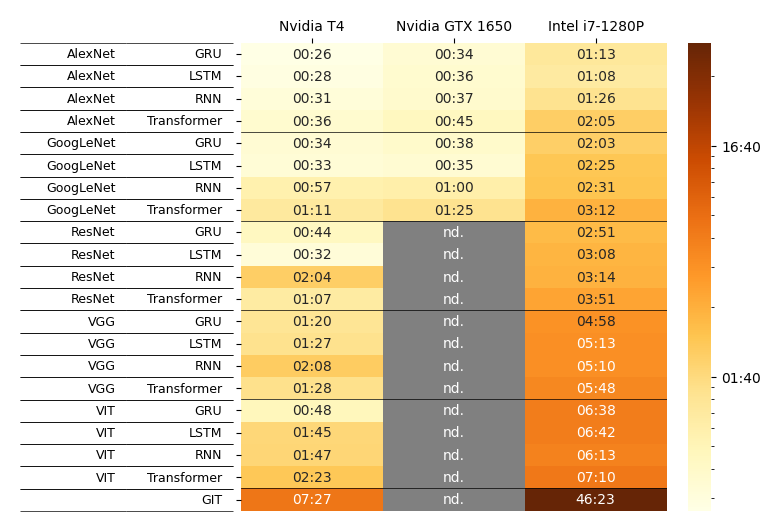
\includegraphics[width=.9\linewidth]{timings/timings_inference_decoders}
  \caption{Czas potrzebny na wygenerowanie podpisów obrazków pochodzących z testowego zbioru danych dla poszczególnych architektur, które zostały wyuczone przy użyciu wcześniej wytrenowanych modułów kodujących. Dane przedstawione w skali logarytmicznej. Opracowanie własne.}
  \label{fig:timings-decoders-inference}
\end{figure}

\begin{figure}[H]
  \centering
  \begin{subfigure}{.5\textwidth}
    \centering
    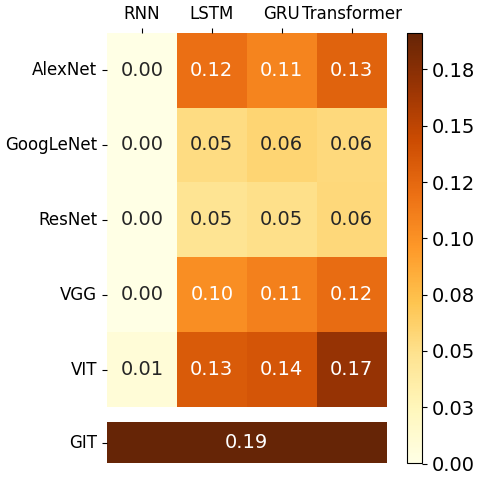
\includegraphics[width=.95\linewidth]{metrics/BLEU}
    \caption{Wartości metryki BLEU}
    \label{fig:bleu}
  \end{subfigure}%
  \centering
  \begin{subfigure}{.5\textwidth}
    \centering
    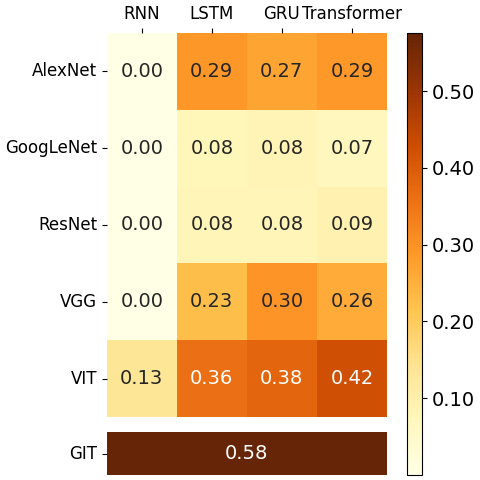
\includegraphics[width=.95\linewidth]{metrics/CIDEr}
    \caption{Wartości metryki CIDEr}
    \label{fig:cider}
  \end{subfigure}%
  \caption{Wartości metryk BLEU oraz CIDEr dla poszczególnych kombinacji modułów kodujących i dekodujących. Opracowanie własne}
  \label{fig:metrics}
\end{figure}

% \begin{table}[H]
% \caption{Czasy potrzebne na wytrenowanie jednej epoki przy pomocy zbioru treningowego oraz czasy potrzebne na wygenerowanie podpisów przy pomocy zbioru testowego dla wszystkich modeli przy użyciu poszczególnych jednostek obliczeniowych. Wartości podane są w formacie: godziny:minuty:sekundy.}\label{times}
% \centering
% \begin{tabular}{lcccccc}
% \hline
% & \multicolumn{2}{c}{GeForce GTX 1650}
% & \multicolumn{2}{c}{Tesla K80}
% & \multicolumn{2}{c}{Intel Core i7-1280P} \\
% \hline
% Model & Trening & Test & Trening & Test & Trening & Test \\
% \hline
% CNN+RNN & 00:16:11 & 00:06:36 & 00:05:18 & 00:05:20 & 00:34:07 & 00:08:40 \\
% CNN+LSTM & 00:16:16 & 00:06:22 & 00:05:40 & 00:05:16 & 00:45:51 & 00:09:45 \\
% CNN+GRU & 00:17:53 & 00:05:36 & 00:05:34 & 00:05:07 & 00:41:26 & 00:08:26 \\
% ResNet50+RNN & 00:28:57 & 00:10:04 & 00:06:44 & 00:06:37 & 01:42:51 & 00:15:23 \\
% ResNet50+LSTM & 00:30:08 & 00:10:17 & 00:06:47 & 00:06:38 & 01:45:08 & 00:14:32 \\
% ResNet50+GRU & 00:31:29 & 00:09:18 & 00:07:05 & 00:06:38 & 01:50:33 & 00:15:17 \\
% VGG16+RNN & nd. & nd. & 00:22:05 & 00:07:01 & 07:55:44 & 00:27:53 \\
% VGG16+LSTM & nd. & nd. & 00:22:35 & 00:06:53 & 10:15:51 & 00:27:26 \\
% VGG16+GRU & nd. & nd. & 00:22:15 & 00:06:52 & 10:02:21 & 00:28:34 \\
% VIT+RNN & nd. & nd. & 00:36:18 & 00:07:15 & 11:38:14 & 00:36:59 \\
% VIT+LSTM & nd. & nd. & 00:36:32 & 00:07:07 & 11:07:06 & 00:37:13 \\
% VIT+GRU & nd. & nd. & 00:36:55 & 00:07:13 & 11:22:54 & 00:36:55 \\
% GIT & nd. & nd. & 00:56:01 & 00:54:47 & 15:31:34 & 08:08:56 \\
% \hline
% \end{tabular}
% \end{table}
